% Last Update: $Id$

\marklabel{sec:OPTSAMBAPOINTANDPRINT:XP}{\section{SAMBA\_LPD - Konfiguration von Point'n'Print unter Windows XP}}

In diesem Abschnitt wird beschrieben, wie die Point'n'Print-Funktionalität mit
Hilfe eines Windows XP-Clients eingerichtet wird.

Zuerst muss der Druckerserver ``gefunden'' werden. Dies kann z.\,B. mit Hilfe
der Netzwerkumgebung erledigt werden
(Abb.~\ref{fig:sambalpd:icon-networking-environment} bis
\ref{fig:sambalpd:networking-environment:4}). Im aktuellen Beispiel heißt die
Arbeitsgruppe ``GARDEN'' und der fli4l-Server ``ODIN''. Der Drucker, für den
Treiber installiert werden sollen, ist ein Brother HL-2240D.

\begin{figure}[hbt!]
\centering

\includegraphics[]{image001}
\caption{Netzwerkumgebung: Symbol auf dem Desktop}
\label{fig:sambalpd:icon-networking-environment}
\end{figure}

\begin{figure}[hbt!]
\centering
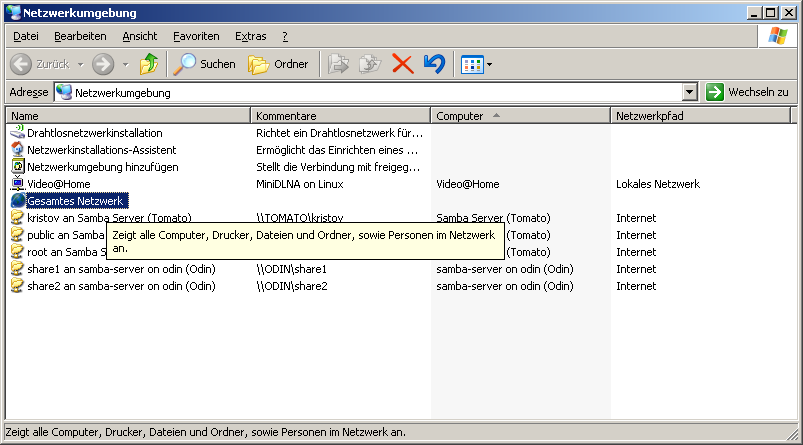
\includegraphics[width=\columnwidth]{image002}
\caption{Netzwerkumgebung: Allgemeine Ansicht}
\label{fig:sambalpd:networking-environment:1}
\end{figure}

\begin{figure}[hbt!]
\centering
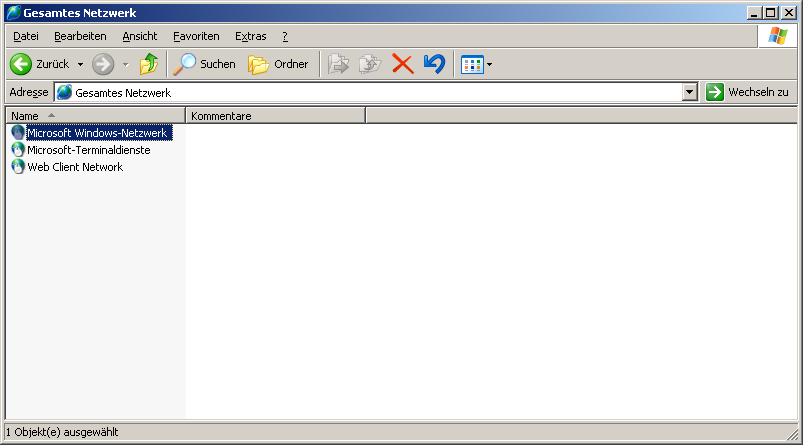
\includegraphics[width=\columnwidth]{image003}
\caption{Netzwerkumgebung: Auswahl des Netzwerk-Typs}
\label{fig:sambalpd:networking-environment:2}
\end{figure}

\begin{figure}[hbt!]
\centering
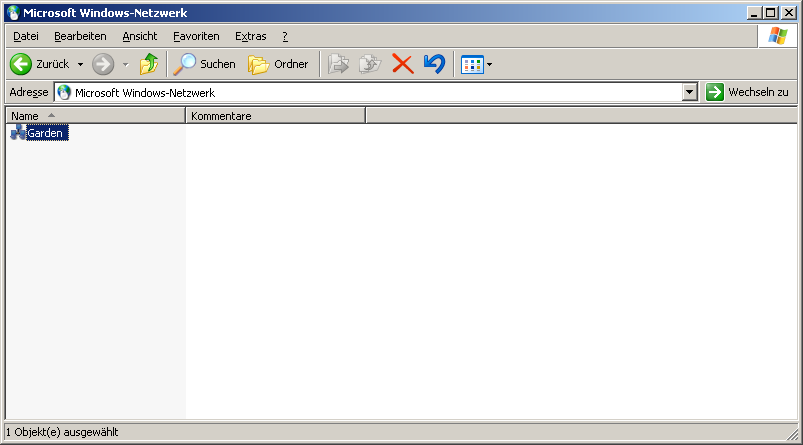
\includegraphics[width=\columnwidth]{image004}
\caption{Netzwerkumgebung: Auswahl der Arbeitsgruppe}
\label{fig:sambalpd:networking-environment:3}
\end{figure}

\begin{figure}[hbt!]
\centering
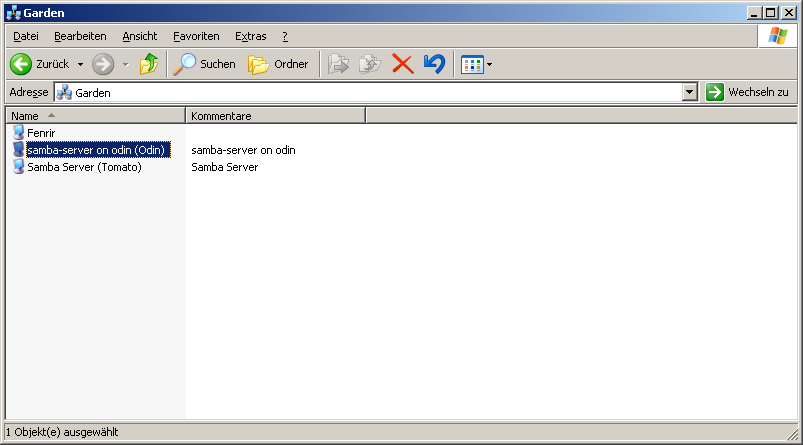
\includegraphics[width=\columnwidth]{image005}
\caption{Netzwerkumgebung: Auswahl des fli4l-Druckerservers}
\label{fig:sambalpd:networking-environment:4}
\end{figure}

Hat man den fli4l-Druckerserver gefunden, so öffnet man durch Doppelklick ein
Fenster, das dessen angebotene Dienste anzeigt
(Abb.~\ref{fig:sambalpd:services}). Dort wählt man ``Drucker und Faxgeräte''
aus. In der folgenden Liste sind alle Drucker zu sehen, die der
fli4l-Druckerserver freigibt. Nun muss der gewünschte Drucker ausgewählt und in
dessen Kontextmenü der Eintrag ``Eigenschaften''
(Abb.~\ref{fig:sambalpd:printerproperties}) ausgewählt werden. Dabei erhält man
eine Meldung (Abb.~\ref{fig:sambalpd:no-driver:1}), dass noch kein Treiber für
diesen Drucker installiert ist (was ja richtig ist). Diese Meldung muss mit
``Nein'' bestätigt werden, da wir den Treiber über eine andere Methode
installieren werden.

\begin{figure}[hbt!]
\centering
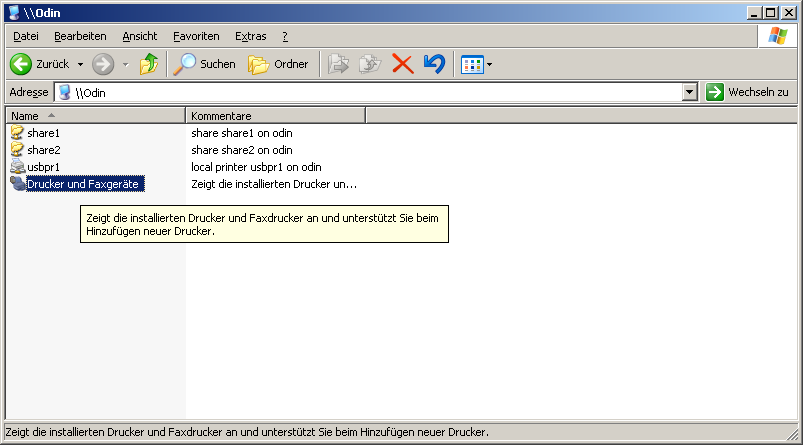
\includegraphics[width=\columnwidth]{image006}
\caption{Serverdienste}
\label{fig:sambalpd:services}
\end{figure}

\begin{figure}[hbt!]
\centering
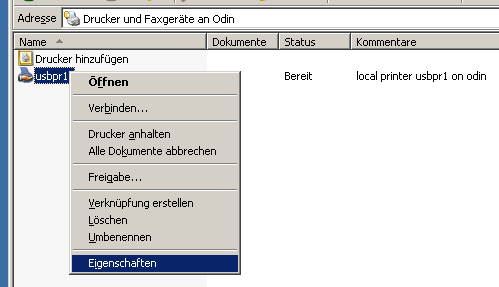
\includegraphics[width=\columnwidth]{image007}
\caption{Auswahl der Drucker-Eigenschaften}
\label{fig:sambalpd:printerproperties}
\end{figure}

\begin{figure}[hbt!]
\centering
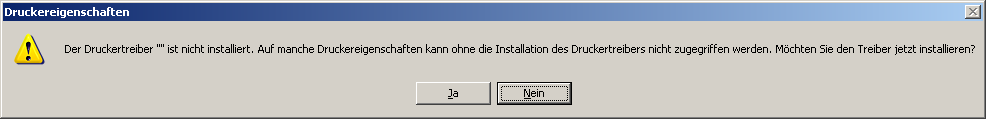
\includegraphics[width=\columnwidth]{image008}
\caption{Druckertreiber fehlt (1)}
\label{fig:sambalpd:no-driver:1}
\end{figure}

Danach öffnet sich der Eigenschaftsdialog. Dort muss man
die Lasche ``Erweitert'' und dort die Schaltfläche ``Neuer Treiber'' auswählen
(Abb.~\ref{fig:sambalpd:props-start-setup}). Dies führt zum Start des
``Assistenten für die Druckerinstallation''
(Abb.~\ref{fig:sambalpd:setup-start}). Mit ``Weiter'' geht es zur
Treiberauswahl (Abb.~\ref{fig:sambalpd:setup-choose-driver:1}). Wenn der
gewünschte Treiber nicht zu finden ist, kann via ``Datenträger'' ein Pfad zu
einem Treiberverzeichnis (das z.\,B.\ auf der Installations-CD des Druckers
liegen kann) angegeben werden; in diesem Falle wird danach nochmal eine zweite
Liste mit den dort verfügbaren Treibern präsentiert, aus der man den Treiber
auswählen muss (Abb.~\ref{fig:sambalpd:setup-choose-driver:2}). Nach erfolgter
Bestätigung der Auswahl über die ``Weiter''-Schaltfläche kommt die Meldung,
dass der Assistent erfolgreich abgeschlossen wurde
(Abb.~\ref{fig:sambalpd:setup-end}). Dies stimmt jedoch nicht, denn erst nach
der Auswahl der ``Fertigstellen''-Schaltfläche wird der Treiber auf den
fli4l-Server kopiert und dort dann aktiviert
(Abb.~\ref{fig:sambalpd:driver-copy}).

\begin{figure}[hbt!]
\centering
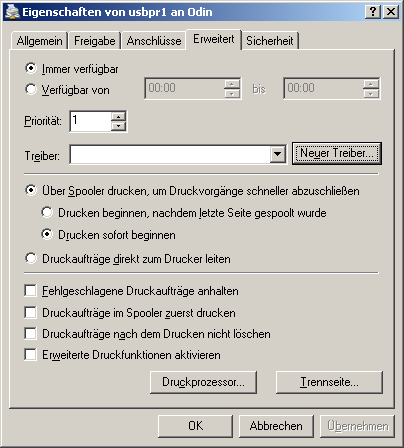
\includegraphics[width=0.8\columnwidth]{image009}
\caption{Druckereigenschaften: Start der Treiberinstallation}
\label{fig:sambalpd:props-start-setup}
\end{figure}

\begin{figure}[hbt!]
\centering
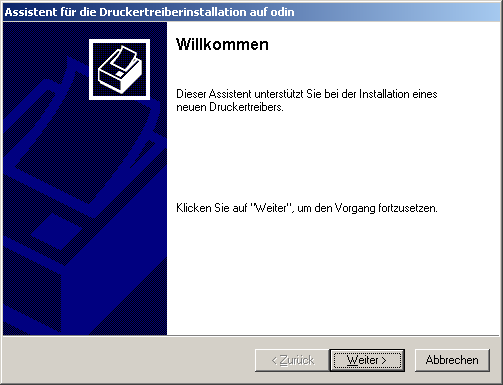
\includegraphics[width=\columnwidth]{image010}
\caption{Druckereigenschaften}
\label{fig:sambalpd:setup-start}
\end{figure}

\begin{figure}[hbt!]
\centering
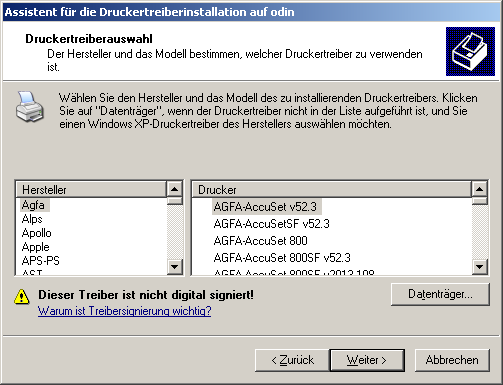
\includegraphics[width=0.7\columnwidth]{image011}
\caption{Treiberinstallation: Treiberauswahl 1}
\label{fig:sambalpd:setup-choose-driver:1}
\end{figure}

\begin{figure}[hbt!]
\centering
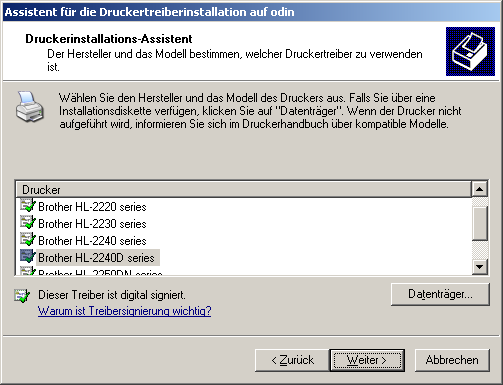
\includegraphics[width=0.7\columnwidth]{image012}
\caption{Treiberinstallation: Treiberauswahl 2}
\label{fig:sambalpd:setup-choose-driver:2}
\end{figure}

\begin{figure}[hbt!]
\centering
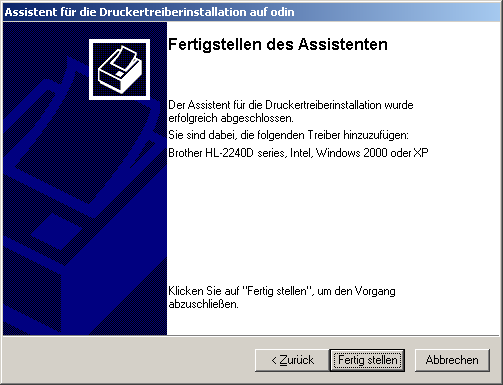
\includegraphics[width=\columnwidth]{image013}
\caption{Treiberinstallation: Abschluss des Assistenten}
\label{fig:sambalpd:setup-end}
\end{figure}

\begin{figure}[hbt!]
\centering
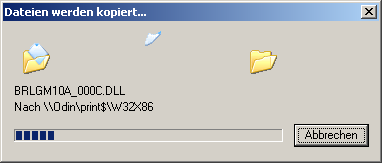
\includegraphics[width=\columnwidth]{image014}
\caption{Treiberinstallation: Kopieren der Treiber}
\label{fig:sambalpd:driver-copy}
\end{figure}

Danach sieht man im Eigenschaften-Dialog, dass der gerade ausgewählte und
installierte Treiber unter ``Treiber'' vermerkt ist
(Abb.~\ref{fig:sambalpd:setup-completed}). Nun muss der Eigenschaften-Dialog
via ``OK'' beendet werden. Dabei bekommt man nochmal eine Meldung, dass der
Treiber fehlt (Abb.~\ref{fig:sambalpd:no-driver:2}), was diesmal Quatsch ist,
weil der Treiber gerade installiert wurde. Deshalb wählt man auch hier mit
``Nein'' wieder aus, dass man jetzt wirklich keinen Treiber installieren will.
Jetzt gelangt man wieder zurück zu der Liste ``Drucker und Faxgeräte'', wobei
Windows den Druckernamen gemäß dem ausgewählten Treiber umbenannt hat
(Abb.~\ref{fig:sambalpd:installed}). Das stellt jedoch kein Problem dar, der
Zugriff auf den fli4l-Druckerserver ist weiterhin möglich.

\begin{figure}[hbt!]
\centering
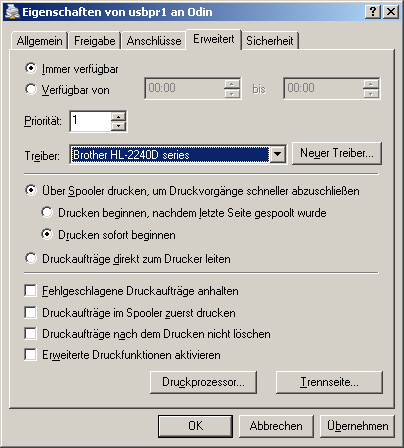
\includegraphics[width=\columnwidth]{image015}
\caption{Treiberinstallation abgeschlossen}
\label{fig:sambalpd:setup-completed}
\end{figure}

\begin{figure}[hbt!]
\centering
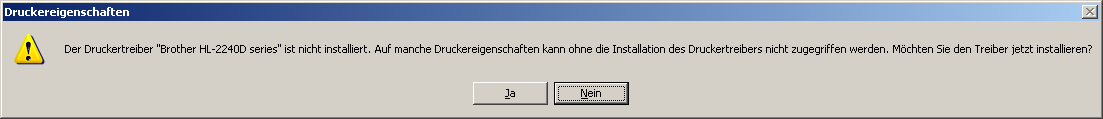
\includegraphics[width=\columnwidth]{image016}
\caption{Druckertreiber fehlt (2)}
\label{fig:sambalpd:no-driver:2}
\end{figure}

\begin{figure}[hbt!]
\centering
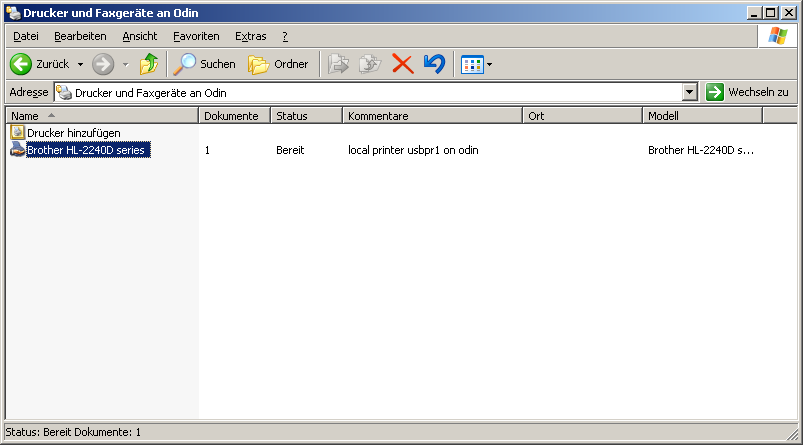
\includegraphics[width=0.8\columnwidth]{image017}
\caption{Teil 1 der Druckerinstallation abgeschlossen}
\label{fig:sambalpd:installed}
\end{figure}

Nun ist man jedoch noch nicht fertig. Denn jetzt müssen die
Standard-Einstellungen des Druckers einmalig gesetzt werden. Dazu geht man
wieder in den Dialog der Drucker-Eigenschaf\-ten
(Abb.~\ref{fig:sambalpd:printerproperties}) und wählt dort in der Lasche
``Erweitert'' die Schaltfläche ``Standardwerte'' aus
(Abb.~\ref{fig:sambalpd:props-reloaded:1}). (Diese Schaltfläche war vorher
noch nicht da, deshalb konnten wir das auch nicht bereits vorhin miterledigen).
Jetzt öffnet sich ein Treiber-abhängiger Dialog
(Abb.~\ref{fig:sambalpd:props-reloaded:2}). In diesem Dialog müssen nun die
gewünschten Druckereinstellungen gesetzt werden. In der Regel muss man das
Papierformat von ``Letter'' auf ``A4'' umstellen. Sollten ausnahmsweise alle
Einstellungen korrekt sein, muss man kurzfristig eine Einstellung verändern und
gleich wieder zurückändern~-- dies ist nötig, damit Windows beim Beenden des
Dialogs via ``OK'' auch wirklich Einstellungen auf dem fli4l-Server speichert.

\begin{figure}[hbt!]
\centering
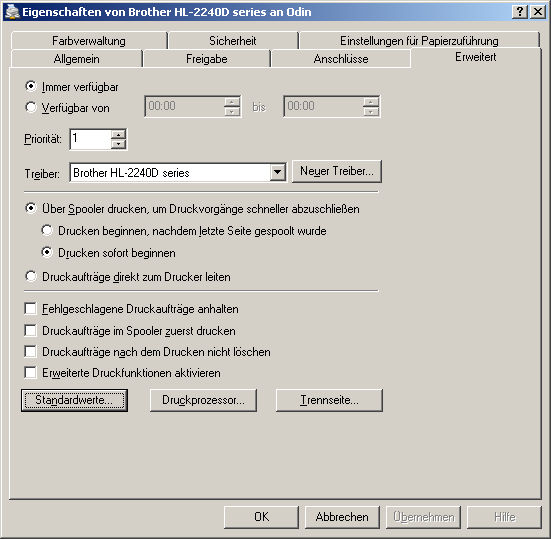
\includegraphics[width=0.8\columnwidth]{image018}
\caption{Setzen der Standardwerte (1)}
\label{fig:sambalpd:props-reloaded:1}
\end{figure}

\begin{figure}[hbt!]
\centering
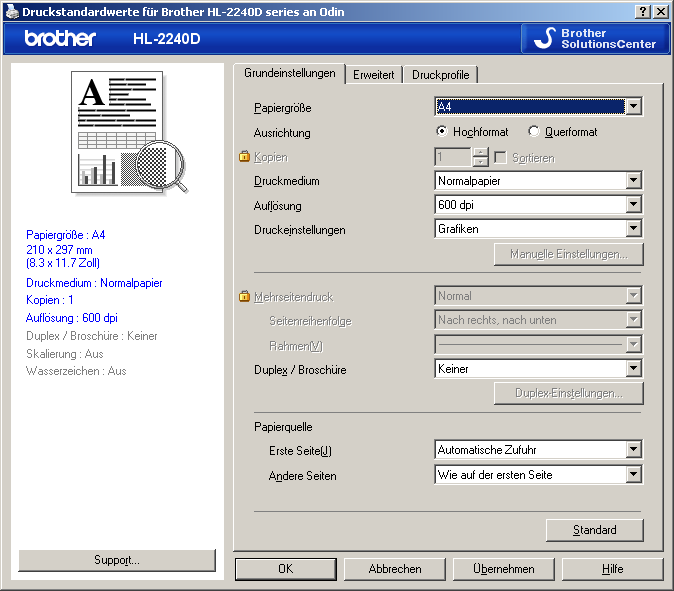
\includegraphics[width=\columnwidth]{image019}
\caption{Setzen der Standardwerte (2)}
\label{fig:sambalpd:props-reloaded:2}
\end{figure}

Nun sind wir am Ziel! Die serverseitige Konfiguration ist abgeschlossen. Will
man jetzt diesen eingerichteten Drucker nutzen, muss man sich mit ihm verbinden
(Abb.~\ref{fig:sambalpd:connect:1}). Die erscheinende Warnmeldung über die
Gefahren der Treiberinstallation (Abb.~\ref{fig:sambalpd:connect:2}) muss man
bestätigen. Danach erscheint der verbundene Drucker in der Druckerumgebung
(Abb.~\ref{fig:sambalpd:printer-environment}). Voilà!

\begin{figure}[hbt!]
\centering
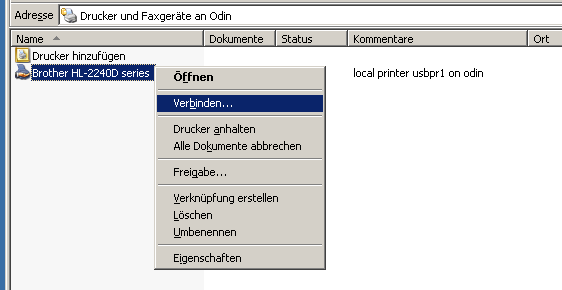
\includegraphics[width=\columnwidth]{image020}
\caption{Verbinden zum Drucker (1)}
\label{fig:sambalpd:connect:1}
\end{figure}

\begin{figure}[hbt!]
\centering
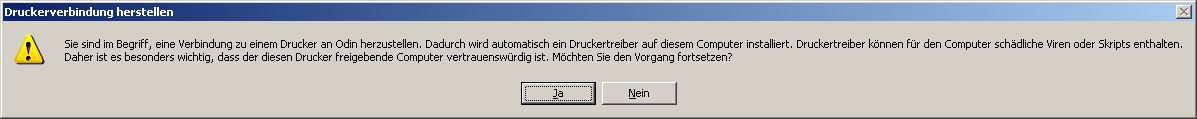
\includegraphics[width=\columnwidth]{image021}
\caption{Verbinden zum Drucker (2)}
\label{fig:sambalpd:connect:2}
\end{figure}

\begin{figure}[hbt!]
\centering
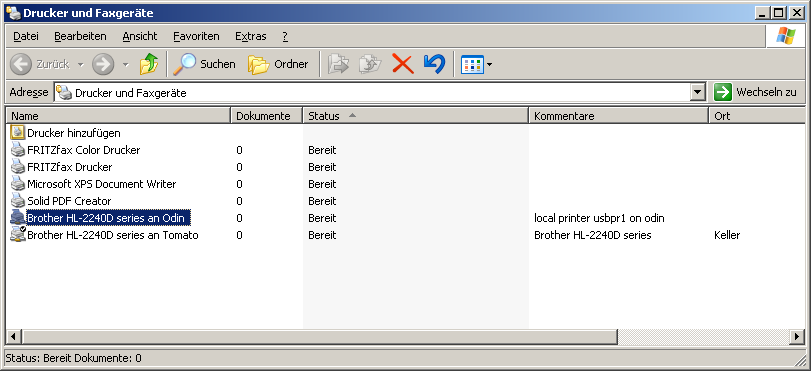
\includegraphics[width=\columnwidth]{image022}
\caption{Verbundener Drucker in der Druckerumgebung}
\label{fig:sambalpd:printer-environment}
\end{figure}
